\documentclass[french]{article}
\usepackage{amssymb, amsmath, mathtools} %pour les mathématiques
\usepackage{fontspec}
\usepackage{xunicode}
\usepackage[a4paper]{geometry}
\usepackage{babel}
\usepackage{hyperref}
\usepackage{pifont}

\newcommand{\cmark}{\ding{51}}%
\newcommand{\xmark}{\ding{55}}%

\newtheorem{post}{Postulat}
\newtheorem{mydef}{Définition}

\begin{document}
\title{Résumé Journalier}
\author{Joffrey Hérard}
\date{\today} 

\maketitle
\section{Les VMs}
\paragraph{Liste de mes connaissances des différentes technologies de virtualisation}
\begin{itemize}
	\item VirtualBox
	\item VMWARE
	\item LXC
	\item Docker
	\item QEMU
	\item KVM
	\item HyperV
	\item Proxmox VE
	\item Oracle VM Server 
	\item Hyper-V Containers
\end{itemize}

Réorganisation des différentes VM par tableau :   
\begin{table}[!h]
\centering
\caption{Différents services de Virtualisations }
\begin{tabular}{|l|l|}
\hline
Conteneurs         & Hyperviseurs Types 1 et 2                                                                              \\ \hline
LXC                & Virtualbox                                                                                             \\
Docker             & VMWare                                                                                                 \\
Vagrant            & Qemu                                                                                                   \\
Hyper-V Containers & \begin{tabular}[c]{@{}l@{}}KVM\\ Proxmox(Basé sur KVM)\\ Oracle VM Server\\ Hyper-V\\\end{tabular} \\ \hline
\end{tabular}
\end{table}
Tout d'abord avant de savoir ce que l'on retiendras on va déjà faire quelque définitions.
\begin{mydef}
Hyperviseur de type 1 : est un logiciel qui s'exécute directement sur une plateforme matérielle ; cette plateforme est alors considérée comme outil de contrôle de système d'exploitation. Un système d'exploitation secondaire peut, de ce fait, être exécuté au-dessus du matériel.
\end{mydef}

\begin{mydef}
Hyperviseur de type 2 : Un hyperviseur de Type 2 est un logiciel qui s'exécute à l'intérieur d'un autre système d'exploitation. Un système d'exploitation invité s'exécutera donc en troisième niveau au-dessus du matériel. Les systèmes d'exploitation invités n'ayant pas conscience d'être virtualisés, ils n'ont pas besoin d'être adaptés.
\end{mydef}

\begin{mydef}
Conteneur/ Isolateur : Un isolateur est un logiciel permettant d'isoler l'exécution des applications dans ce qui est appelé des contextes.L'isolateur permet ainsi de faire tourner plusieurs fois la même application dans un mode multi-instance, mais les environnements virtualisés ne sont pas complètement isolés.Cependant on ne peut pas vraiment parler de virtualisation de systèmes d’exploitation. 
\end{mydef}

\paragraph{Quoi garder?}
Choix sur les différentes VM :  
\begin{table}[!h]
\centering
\begin{tabular}{lll}
LXC   \checkmark \par           & Docker  \checkmark \par            &  HyperV \xmark \\
VMWare  \xmark         & VirtualBox   \checkmark \par       & Qemu \xmark   \\
Oracle VM Server \xmark & Proxmox  \cmark          & KVM \xmark    \\
Hyper-V Containers \xmark          &  &
\end{tabular}
\end{table}
Justification des choix cas par cas :
\begin{post}
LXC : Gestionnaire de Conteneurs Linux, je l'ai utilisé aussi souvent que Docker (NB : Docker basé sur LXC)
\end{post}


\begin{post}
Docker : Gestionnaire de Conteneurs, que j'ai utilisé très souvent. (NB : Docker basé sur LXC)
\end{post}

\begin{post}
VirtualBox : Utilisé de manière courante aussi, de plus c'est un Hyperviseur classique de Type 2.
\end{post}

\begin{post}
Proxmox VE : Utilisé d'un point de vue utilisateur, mais il complète la liste en étant un Hyperviseur de type 1.
\end{post}

\begin{post}
VMware : Je ne sais pas si l'on a une licence à notre disposition ? 
\end{post}

\begin{post}
Qemu : Utilisé quelque fois cependant, basé sur KVM(Comme Proxmox VE) et XEN(Connu que de nom). 
\end{post}


\begin{post}
Oracle VM Server : Jamais abordé ..et je ne sais pas si l'on a une licence à notre disposition ? 
\end{post}

\begin{post}
KVM : HyperViseur de type 1. Proxmox étant basé sur KVM et étant lui aussi un Hyperviseur de Type 1, 
\end{post}

\begin{post}
Hyper-V Containers : Jamais abordé .. ne connaissait pas son existence avant de faire de la recherche sur le sujet .
\end{post}

\begin{post}
Hyper-V : Jamais abordé.
\end{post}

\newpage
\section{Les tests}
\paragraph{Test de performance}
 Les informations recueillies concernent les temps de réponse utilisateurs, les temps de réponse réseau et les temps de traitement d’une requête.
\paragraph{Test de montée en charge}
Il s'agit d'un test au cours duquel on va simuler un nombre d'utilisateurs sans cesse croissant de manière à déterminer quelle charge limite le système est capable de supporter
\paragraph{Test de dégradations}
 Ce test peut tenir compte ou non de la cadence des itérations, la représentativité en termes d'utilisateurs simultanés vs. sessions simultanées n'étant pas ici un objectif obligatoire, s'agissant ici plutôt de déterminer les points de contention générés par chaque scénario fonctionnel.
\paragraph{Test de robustesse}
 il s'agit de tests au cours desquels on va simuler une charge importante d'utilisateurs sur une durée relativement longue, pour voir si le système testé est capable de supporter une activité intense sur une longue période sans dégradations des performances et des ressources applicatives ou système.
\paragraph{Test aux limites} 
Proche du test de capacité,
\paragraph{Benchmark}
Un benchmark est un logiciel "banc d'essai" permettant de mesurer les performances d'un système pour le comparer à un autre. Ces test doivent donc être équivalents, en conditions similaires, seul les résultats peuvent changer.
\newpage
\section{Retour sur la liste des choses à faire}

\paragraph{Retour sur le point 3}

En réalité, j'ai mis les use case à cette place, mais sur le schéma de la page suivante on voit que il ce fait en "parallèle ".Mais effectivement on pourrais le mettre en première positions puis faire l'ensemble des autres tache à faire.
J'ai donc mis à jour ce correctif dans le graphe du précédent rapport journalier. 
\paragraph{Retour sur le point 6}
Parce que à ma connaissance, il y a probablement plusieurs éléments (A entendre différent services  )déjà installer, et sachant que l'on doit faire des tests, il est nécessaire de "nettoyer la machine" afin de n'avoir que ce qui est utile à nos besoins, et pas avoir des Démons qui s’exécutent et donc utilisent des ressources. 
\paragraph{Retour sur le point 7 } 
\subparagraph{Pourquoi une sonde neutre}
Car les relevés feront objets de statistique on pourrait en sortir des données aberrant si la sonde influe elle même sur son propre relevé. Statistiquement si cette influence est constante elle peut en être extraite. 
\subparagraph{Pourquoi une sonde interne ?}
La encore Interne a quoi ? interne a chaque machine virtuelle/ Conteneurs ?
Si on part sur le fait que il y ai une sonde sur chaque machines virtuelles crée. 
\begin{itemize}
	\item Si le nombre des machines virtuelle/ conteneurs tend vers l'infinie ça veut dire que le nombre de sonde est infinie lui aussi ? Il y a donc un besoin de répartitions et de récupération des données fournies par les sondes.
	\item Par contre si on exécute plusieurs machines virtuelles différentes, par exemple  50 Windows 20 Ubuntu 30 CentOS, il faut être capable de différencier les relevés d'une machine par rapport à une autre avec un ensemble d'informations qui reste à définir...
	\item Différenciation point à point de chaque relevé $\rightarrow$ On peut faire une structure de distribution des relevés si on le fait ainsi par exemple en prenant une architecture de fat-tree
Ceci dit on interpréterait chaque nœud, comme une sonde qui soit communique avec une autre sonde soit "sonde" justement une machines.
\begin{figure}[!h]
\centering
\caption{Fat tree}
	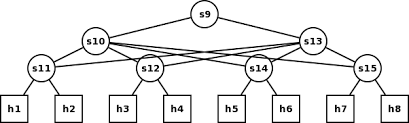
\includegraphics[scale=0.5]{fat.png}
\end{figure}
\end{itemize}
\subparagraph{Pourquoi une sonde externe  ?}
L’Intérêt serait d'avoir un seul gros amas de données en même endroit il ne resterait que à	en extraire les informations désiré, par contre le temps de recherche peut etre long, plus il y a de donnée enregistrés( encore une fois cela reste à définir) il y aurait cependant un enregistrement qui serait par transmission d'information, un aspect Moniteur d'informations pour chaque vm a mettre en place ? 

\newpage
\paragraph{Retour sur le point 8 a) }
\subparagraph{Préparation de la machines physiques }
Une remise a zéro pour ne pas faussez les résultats/comparaisons, il faut une base identique, pour une neutralité de la base il faut que l'on parte du même constat pour toutes les technologies aue on compareras . 
\subparagraph{Préparation des machines virtuelles }
Il faudra probablement préparé des scripts de lancement de machines virtuelles pour nous en donné une certaine quantités (A déterminé ).
\paragraph{Retour sur le point 8 c }
Si l'on suppose que tout est parfait, effectivement il n'y pas forcément besoin de surveiller régulièrement ! 
Par contre savoir ou le test en ai si il y a eu un crash d'une VM, l'idée serait de mettre un message dans un fichier.log pour savoir si des services se sont arrêter et surtout que on avait pas prévu . 

\paragraph{Listes des choses à faire Mis a jour 4/04/2017}
\begin{enumerate}
	\item Définitions des cas d'utilisations. 
	\item Choix des Hyperviseurs de Type 1 ? Type 2 ? Conteneurs?
	\item Choix cible des Tests.
	\item Définitions des différents scenarios associé au différent schéma ..
	\item Préparations des différents scripts associés aux scenarios pour les différent hyperviseur, conteneurs 
	\item Remise à zero de la machine hôte.
	\item Mise en place d'une << sonde >> pour effectué les relevés de sorte à être des plus neutre dans les enregistrements.
	\item Mise en place des Tests 
		\begin{enumerate}
			\item Préparations de la machine physique et des machines virtuelles. 
			\item Lancement des tests.
			\item Surveillance régulière du bon déroulement des différents test.
			\item Récupérations des données . 
			\item Analyse des résultats sur la cohérence .
			\begin{enumerate}
				\item Établir des liens entre certain paramètres $\rightarrow $ les confirmers par d'autre test ? 
				\item Analyse sur les différents hyperviseur/conteneurs sur les mêmes scenarios 
			\end{enumerate}
			\item Représentations des résultats pour chaque batterie de tests. (Courbes) et les interprétations.
			\item Retour à l’étape (a) si nécessaire sinon étapes suivantes.
		\end{enumerate}
	\item Écriture du rapport au fur et mesure.	
			
\end{enumerate}




\newpage
\begin{figure}[!h]
\centering
\caption{Graphe des dépendances }
\label{Graphe des dépendances }
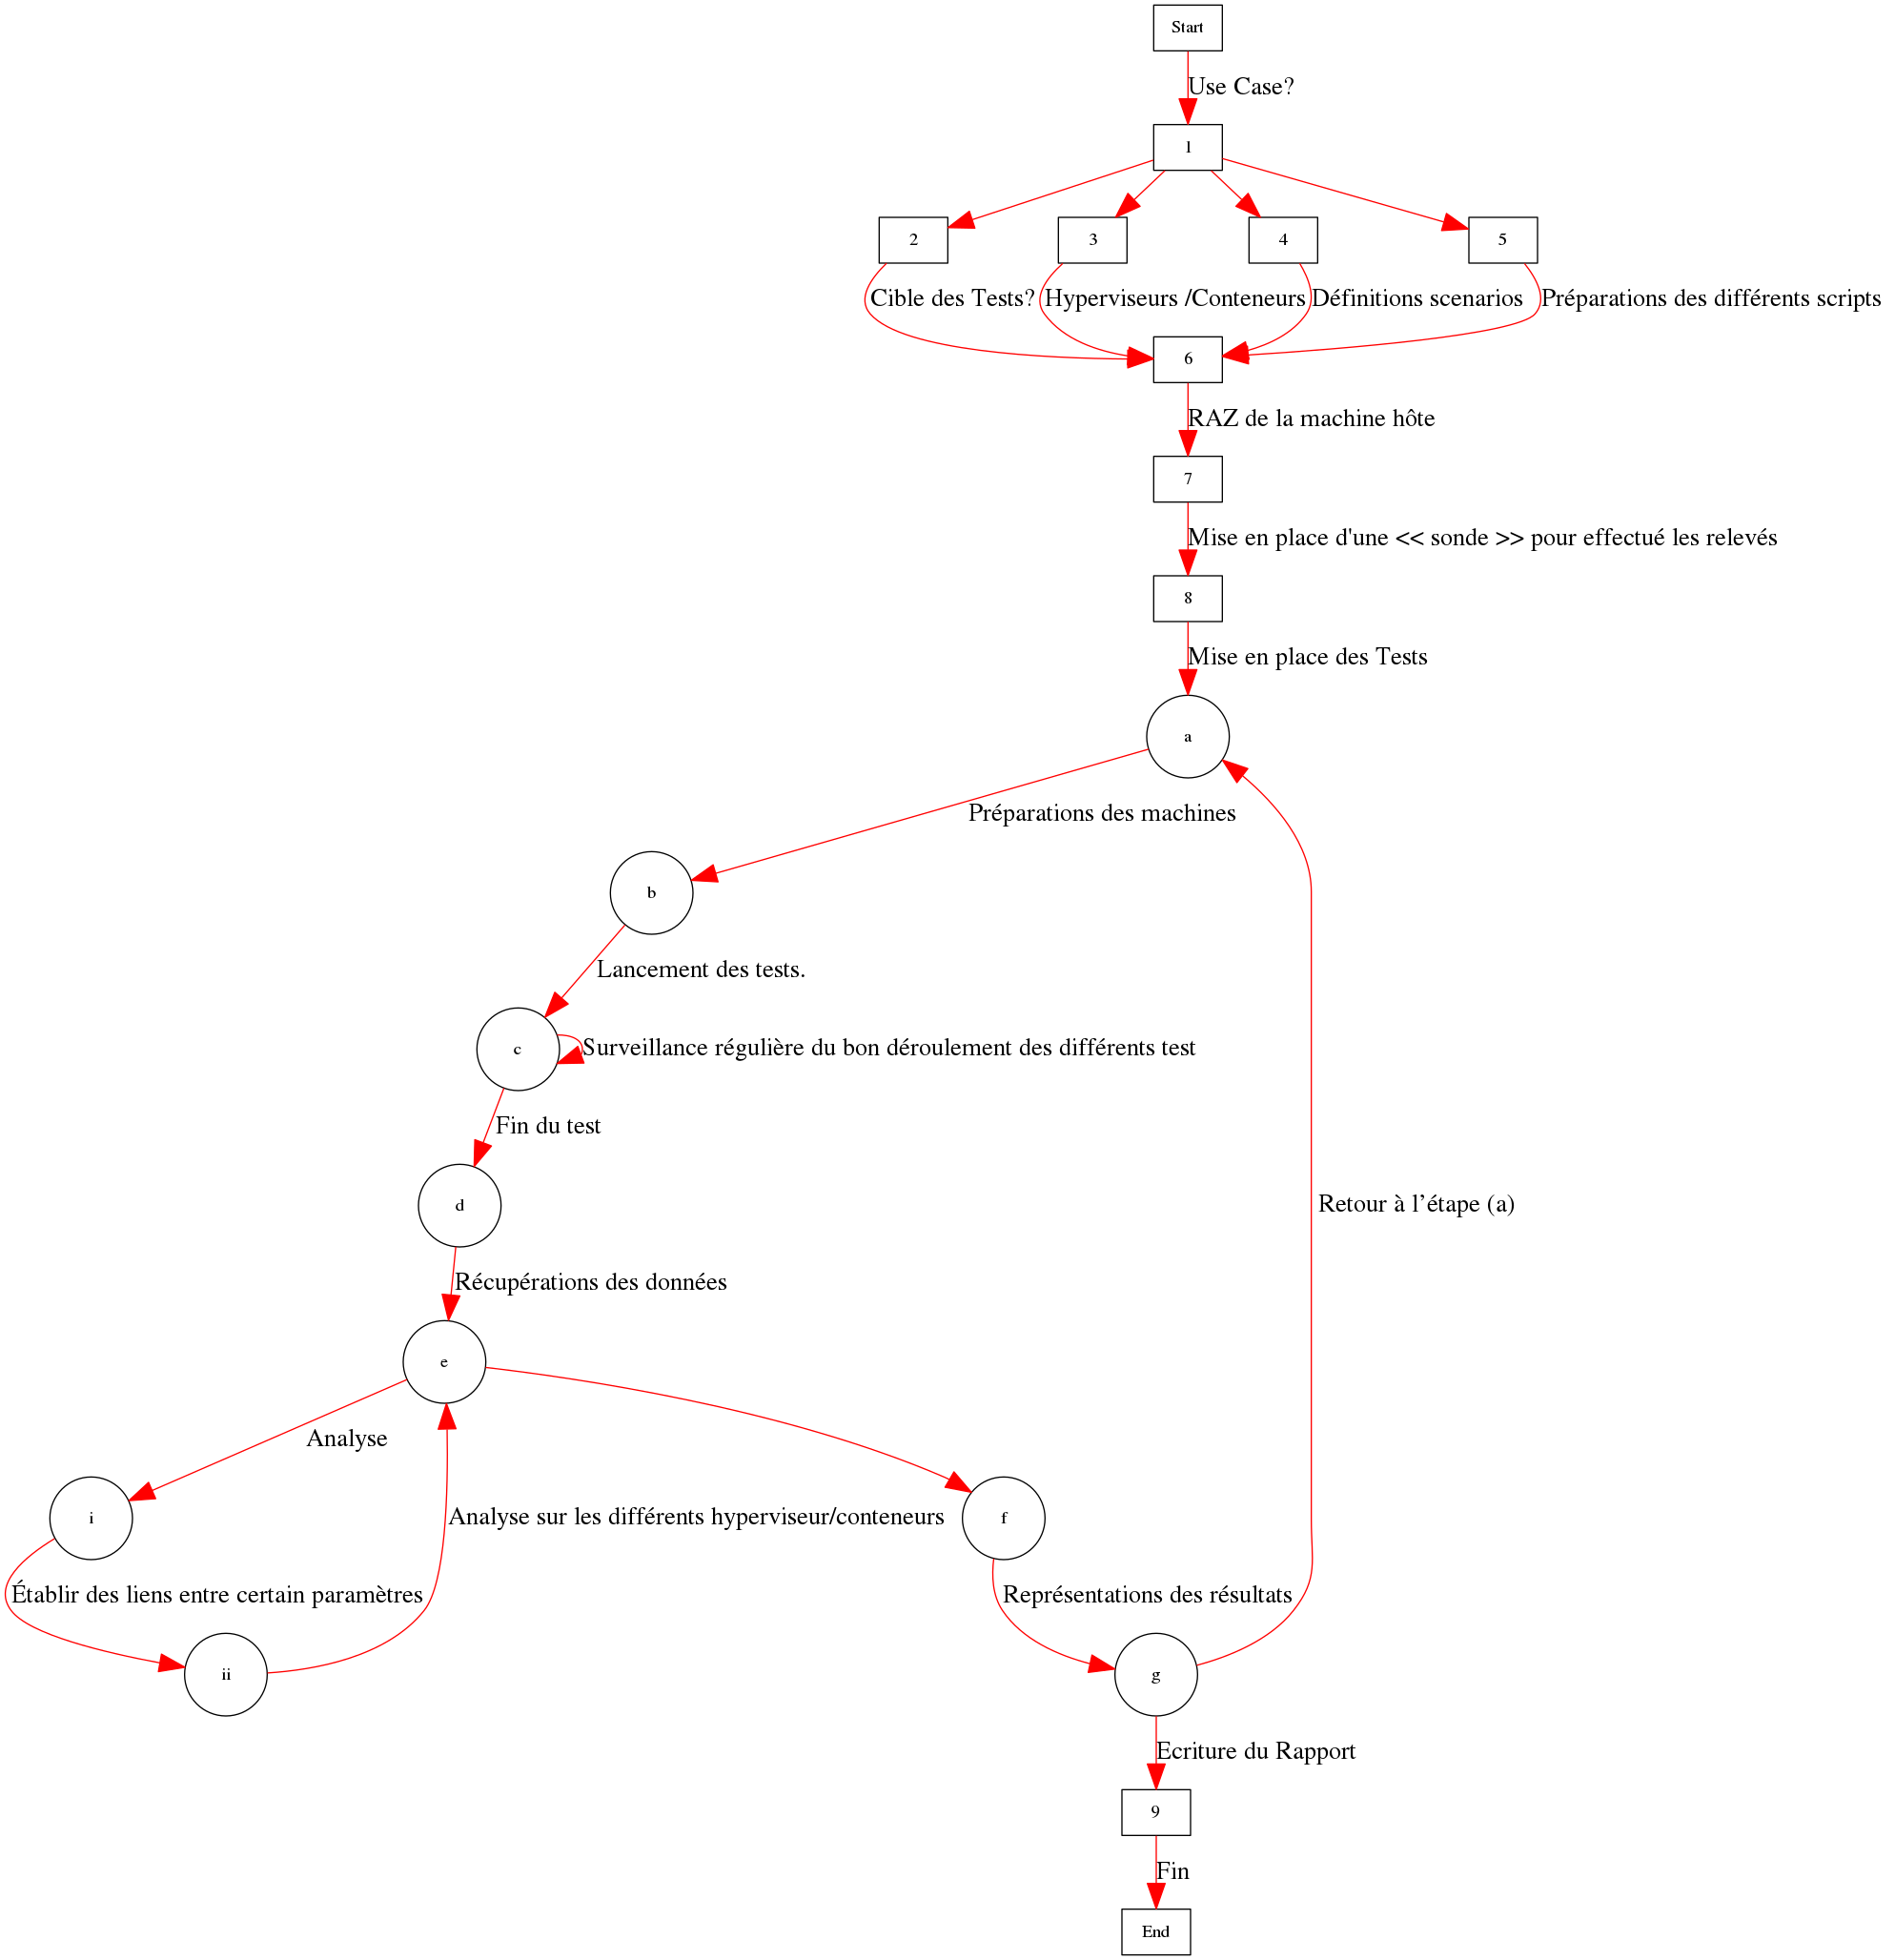
\includegraphics[scale=0.250]{GrapheDepends.png}
\end{figure}


\newpage
\begin{thebibliography}{9}

   \bibitem{Docker}
          Documentation Docker
          \url{https://docs.docker.com/}.
   \bibitem{HyperV Conteneurs}
          Hyper-V Containers
          \url{https://docs.microsoft.com/en-us/virtualization/windowscontainers}.
   \bibitem{Linux containers}
         Linux Containers
         \url{https://linuxcontainers.org/fr/}.
   \bibitem{Virtual Box}
         Virtual Box
         \url{ https://www.virtualbox.org/}.
   \bibitem{Proxmox VE}
         Proxmox VE
         \url{https://www.proxmox.com/en/}.
   \bibitem{VmWare}
         VmWare
         \url{ http://www.vmware.com/fr.html}.
   \bibitem{QEMU}
         QEMU
         \url{http://www.qemu-project.org/   }.
   \bibitem{Hyper-V}
         Hyper-V
         \url{https://www.microsoft.com/fr-fr/cloud-platform/server-virtualization}.      
   \bibitem{KVM}
         KVM
         \url{https://www.linux-kvm.org/}.
   \bibitem{Wikipedia-Test}
         Wikipedia sur les Tests
         \url{https://fr.wikipedia.org/wiki/Test_de_performance}.
   \bibitem{VMMark}
         VM Mark
         \url{https://www.vmmark.com/products/vmark.html}. 
   \bibitem{VM history}
         VM history par IBM
         \url{http://www.vm.ibm.com/history/ }.
               
\end{thebibliography}


\end{document}